\documentclass{beamer}
\usetheme{Boadilla}
\usecolortheme{beaver}

\usepackage[german]{babel}
\usepackage[utf8x]{inputenc}
\usepackage{tabularx}
\usepackage{slashbox}
\usepackage{tikz}
\usetikzlibrary{mindmap,trees}

\title[Collaborative \& transparent FS development]{Collaborative and transparent Free Software development} 
\author{Lydia Pintscher} 
\institute[KIT]{Institute of Applied Informatics and Formal Description Methods\\
Karlsruhe Institute of Technology
}
\date{\today}

\begin{document}
\begin{frame}
\titlepage
\end{frame}

\section*{\"Ubersicht}

\begin{frame}
\frametitle{\"Ubersicht}
\tableofcontents
\end{frame}

\section{Einleitung}

\begin{frame}
\frametitle{Einleitung}
\begin{itemize}
 \item Freie Software ist heute ein integraler Bestandteil der Technologiewelt
 \item sehr unterschiedliche Projekte mit \"ahnlichen Problemen: Amarok und Halo
 \item mehr Transparenz und Kollaboration
 \item Analyse und Verbesserung des Entwicklungsprozesses mit bekannten Tools
\end{itemize}
\end{frame}

\section{Grundlagen}

\begin{frame}
\frametitle{Kollaboration und Transparenz}
\begin{itemize}
 \item Kollaboration: ``working jointly with others or together especially in an intellectual endeavour'' (Merriam-Webster)
 \item Transparenz (hier): einfacher Zugang zu und Sichtbarkeit von Informationen 
\end{itemize}
\end{frame}

\begin{frame}
\frametitle{Freie Software (1)}
\begin{itemize}
 \item beschreibt eine Philosophy zum Entwickeln und Verbreiten von Software
 \item 4 Freiheiten (FSF):
    \begin{enumerate}
      \item Die Freiheit, das Programm für jeden Zweck zu benutzen.
      \item Die Freiheit, zu verstehen, wie das Programm funktioniert und wie man es für seine Ansprüche anpassen kann.
      \item Die Freiheit, Kopien weiterzuverbreiten, so dass man seinem Nächsten weiterhelfen kann.
      \item Die Freiheit, das Programm zu verbessern und die Verbesserungen der Öffentlichkeit zur Verfügung zu stellen, damit die ganze Gemeinschaft davon profitieren kann.
    \end{enumerate}
 \item bekannnte Beispiele: Apache, Firefox, MediaWiki
\end{itemize}
\end{frame}

\begin{frame}
\frametitle{Freie Software (2)}
\begin{itemize}
 \item verschiedene Projektformen m\"oglich (volunteer $\leftrightarrow$ company)
 \item verschiedene Gr\"unde teilzuhaben (extrinsisch $\leftrightarrow$ intrinsisch)
 \item unterschiedlich gro\ss e gef\"uhlte Distanz zwischen Mitgliedern
 \item unterschiedliche Arbeits- und Kommunikationsstile
\end{itemize}
\begin{figure}[h]
	\centering
	\begin{tikzpicture}
		\draw (0cm, 0cm) -- (10cm, 0cm);
		\foreach \x in {0, 1, 2, 3, 4, 5, 6, 7, 8, 9, 10} \draw (\x cm, 3pt) -- (\x cm, - 3pt);
		\draw (0cm, 0cm) node[below=5pt] {volunteer};
		\fill (0.625cm, 0cm) circle (2pt);\draw (0.625cm, 0cm) node[above=5pt] {Amarok};
		\draw (5cm, 0cm) node[below=5pt] {gemischt};
		\fill (8.75cm, 0cm) circle (2pt);\draw (8.75cm, 0cm) node[above=5pt] {Halo};
		\draw (10cm, 0cm) node[below=5pt] {bezahlt};
	\end{tikzpicture}	\caption{Spektrum der bestimmenden Kr\"afte in einem Freien Software Projekt}
	\label{spectrumofprojectdriver}
\end{figure}
\end{frame}

\begin{frame}
\frametitle{Halo}
\begin{itemize}
 \item Erweiterungen f\"ur Semantic MediaWiki
 \item Vereinfachung und Erweiterung der Nutzung semantischer Daten in einem Wiki
 \item Hauptaugenmerk auf Nutzung im Gesch\"aftsumfeld
 \item sehr starker Einfluss von Hauptsponsor Vulcan Inc.
 \item Atmostph\"are in der Community stark gezeichnet von kommerziellem Einfluss
\end{itemize}
\end{frame}

\begin{frame}
\frametitle{Amarok}
\begin{itemize}
 \item Musikabspielprogramm aus der KDE Community
 \item fast ausschlie\ss lich volunteer-driven
 \item Motto: rediscover your music
 \item verteiltes Team - Kommunikation \"uber IRC und Mailinglisten
 \item sehr flache Teamstruktur
\end{itemize}
\end{frame}

\section{Analyse des aktuellen Entwicklungsprozesses}

\begin{frame}
\frametitle{Analyse des aktuellen Entwicklungsprozesses}
\begin{itemize}
 \item strukturierte, vertrauliche Interviews um herauszufinden wer die Beteiligten sind, welche Tools benutzt werden und welche Probleme bew\"altigt werden m\"ussen
 \item Auswahl der Teilnehmer basierend auf ihrer Zeit im Projekt und ihrem T\"atigkeitsbereich
\end{itemize}
\begin{figure}[h!]
 \centering
 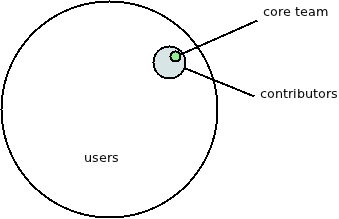
\includegraphics[scale=0.35,keepaspectratio=true]{./communitymodel.png}
\end{figure}
\end{frame}

\begin{frame}
\begin{figure}[h!]
 \centering
 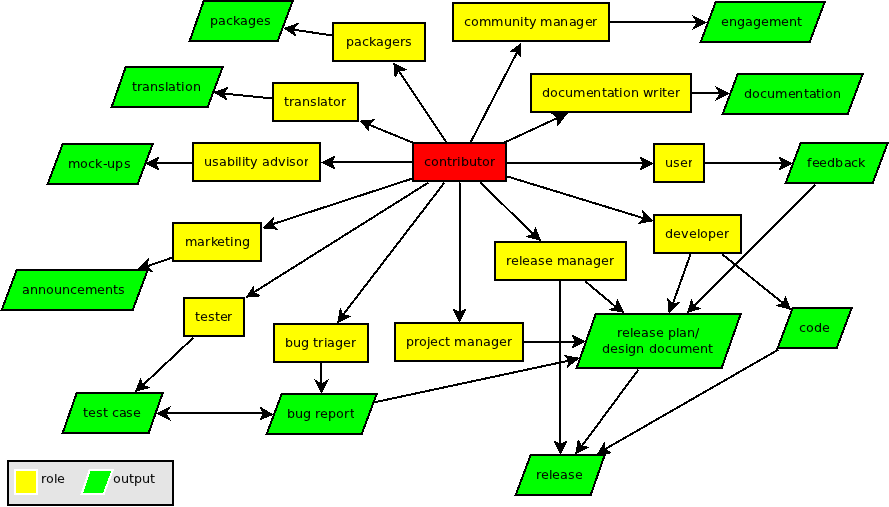
\includegraphics[scale=0.35,keepaspectratio=true]{./ontology.png}
\end{figure}
\end{frame}

\subsection{Halo}

\begin{frame}
\frametitle{Halo}
\begin{figure}[h!]
 \centering
 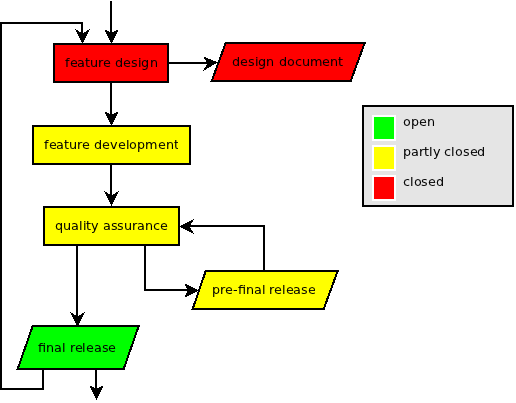
\includegraphics[scale=0.5,keepaspectratio=true]{./ReleaseProcessHalo.png}
\end{figure}
\end{frame}

\begin{frame}
\frametitle{Halo}
\begin{center}
\begin{tikzpicture}
  \path[small mindmap, concept color=green, text=black]
    node[concept] {Halo activities}
    [clockwise from=0]
    child[concept color=green!80, grow=0] {
      node[concept] {feature design}
    }  
    child[concept color=green!80, grow=60] {
      node[concept] {writing code}
    }
    child[concept color=green!80, grow=120] {
      node[concept] {quality assurance}
    }  
    child[concept color=green!80, grow=180] {
      node[concept] {user engagement and support}
    }
    child[concept color=green!80, grow=240] {
      node[concept] {contributor engagement}
    }  
    child[concept color=green!80, grow=300] {
      node[concept] {promotion}
    };
\end{tikzpicture}
\end{center}
\end{frame}

\begin{frame}
\frametitle{Halo}
\begin{center}
\begin{tikzpicture}
  \path[small mindmap, concept color=green, text=black]
    node[concept] {Halo problems}
    [clockwise from=0]
    child[concept color=green!80, grow=0] {
      node[concept] {com\-mu\-ni\-ca\-tion of vision/goal}
    }  
    child[concept color=green!80, grow=90] {
      node[concept] {co\-or\-di\-na\-tion of QA}
    }
    child[concept color=green!80, grow=180] {
      node[concept] {trans\-par\-en\-cy and co\-or\-di\-na\-tion}
    }  
    child[concept color=green!80, grow=270] {
      node[concept] {user input}
    };
\end{tikzpicture}
\end{center}
\end{frame}

\subsection{Amarok}

\begin{frame}
\frametitle{Amarok}
\begin{figure}[h!]
 \centering
 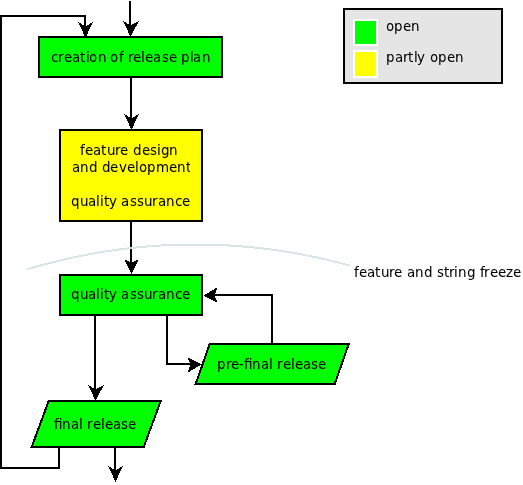
\includegraphics[scale=0.43,keepaspectratio=true]{./ReleaseProcessAmarok.png}
\end{figure}
\end{frame}

\begin{frame}
\frametitle{Amarok}
\begin{center}
\begin{tikzpicture}
  \path[small mindmap, concept color=blue, text=white]
    node[concept] {Amarok activities}
    [clockwise from=0]
    child[concept color=blue!80, grow=0] {
      node[concept] {release management}
    }  
    child[concept color=blue!80, grow=60] {
      node[concept] {writing code}
    }
    child[concept color=blue!80, grow=120] {
      node[concept] {quality assurance}
    }  
    child[concept color=blue!80, grow=180] {
      node[concept] {user engagement and support}
    }
    child[concept color=blue!80, grow=240] {
      node[concept] {team engagement and management}
    }  
    child[concept color=blue!80, grow=300] {
      node[concept] {promotion}
    };
\end{tikzpicture}
\end{center}
\end{frame}

\begin{frame}
\frametitle{Amarok}
\begin{center}
\begin{tikzpicture}
  \path[small mindmap, concept color=blue, text=white]
    node[concept] {Amarok problems}
    [clockwise from=0]
    child[concept color=blue!80, grow=0] {
      node[concept] {clear vision/goal}
    }  
    child[concept color=blue!80, grow=90] {
      node[concept] {road map}
    }
    child[concept color=blue!80, grow=180] {
      node[concept] {trans\-par\-en\-cy and co\-or\-di\-na\-tion}
    }  
    child[concept color=blue!80, grow=270] {
      node[concept] {co\-or\-di\-na\-tion of QA}
    };
\end{tikzpicture}
\end{center}
\end{frame}

\subsection{Vergleich und Schlussfolgerung}

\begin{frame}
\frametitle{Vergleich und Schlussfolgerung}
\begin{tabularx}{\textwidth}{|X|X|X|}
\hline
 & Halo & Amarok \\
\hline \hline
Alter & 2 Jahre & 7 Jahre \\
\hline
Programmiersprache & PHP & C++ \\
\hline
Motivation & vorw. extrinsisch & vorw. intrinsisch \\
\hline
Teamgrenzen & klar & unklar\\
\hline
haupts\"achlich genutzte Medien & pers\"onlich, Mailinglisten, Bugreports & IRC, Mailinglisten \\
\hline
Community au\ss erhalb des Kernteams & klein & gro\ss \\
\hline
Offenheit & rel. geschlossen & rel. offen \\
\hline
``release early release often'' & nein & ja \\
\hline
Planung & viel & sehr wenig \\
\hline
Richtungsvorgabe & Management/Team & individuelle Entwickler \\
\hline
Standort Kernteam & Deutschland & weltweit \\
\hline
\end{tabularx}
\end{frame}

\begin{frame}
\frametitle{Vergleich und Schlussfolgerung}
\begin{tabularx}{\textwidth}{|X|X|X|}
\hline
 & Halo & Amarok\\
\hline \hline
Versionskontrollsystem & SVN & git\\
\hline
wiki & MediaWiki, SMW und Halo & MediaWiki\\
\hline
bug tracker & Bugzilla & Bugzilla\\
\hline
build server & Hudson & Hudson\\
\hline
test case management & TestLink & Seite im wiki\\
\hline
\end{tabularx}
\end{frame}

\section{Design eines verbesserten Entwicklungsprozesses}

\begin{frame}
\frametitle{Design eines verbesserten Entwicklungsprozesses}
foo
\end{frame}

\begin{frame}
\frametitle{Anforderungen, Erwartungen und Rahmenbedingungen}
\begin{itemize}
 \item Vertrauen aufbauen durch Transparenz
 \item schnellen \"Uberblick und Beitr\"age gew\"ahren
 \item ``cookie licking'' vermeiden
 \item keine Zeit verschwenden
 \item Freie Software nutzen
 \item Erwartungen richtig setzen
 \item Einstellungen \"andern
\end{itemize}
\end{frame}

\begin{frame}
\frametitle{Kollaborativ in einem Team arbeiten}
\begin{itemize}
 \item Team und Taskawareness
 \item Release schedule
 \item Code ownership
 \item Checklisten
 \item Vertrauen aufbauen durch Einbeziehen
 \item Commits verkn\"upfen
\end{itemize}
\end{frame}

\begin{frame}
\frametitle{Kollaborativ an einer Vision arbeiten}
\begin{itemize}
 \item Erstellen und Kommunizieren einer Vision
 \item Kollaborativ eine Vision aktualisieren
\end{itemize}
\end{frame}

\begin{frame}
\frametitle{Kollaborativ eine Roadmap erstellen}
\begin{columns}
 \column{.4\textwidth}
  \begin{itemize}
   \item Lebenszyklus eines Feature requests
   \item Umfang und Schwierigkeit von Feature requests
   \item Erwartungen um einen Feature request kommunizieren
   \item Claiming und Zuweisen von Feature requests
   \item Feature request Seite und \"Ubersicht
  \end{itemize}
 \column{.6\textwidth}
  \begin{figure}[h!]
   \centering
   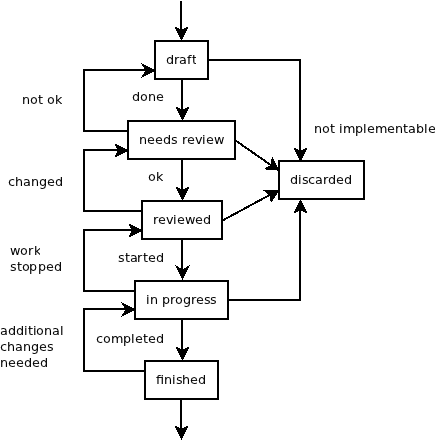
\includegraphics[scale=0.4,keepaspectratio=true]{./featurerequeststates.png}
  \end{figure}
\end{columns}
\end{frame}

\begin{frame}
\frametitle{Kollaborativ eine Roadmap erstellen}
\begin{table}[h]
\begin{tabular}{|p{0.1\textwidth}|p{0.8\textwidth}|}
\hline
Priority & Meaning\\
\hline \hline
P1 & will be implemented by the core team\\
\hline
P2 & will potentially be implemented by the core team\\
\hline
P3 & will not be implemented by the core team but patches will be happily accepted\\
\hline
P4 & undecided or disputed\\
\hline
P5 & will not be implemented and patches will likely not be accepted into the main repository\\
\hline
\end{tabular}
\centering
\end{table}
\end{frame}

\begin{frame}
\frametitle{Kollaborativ eine Roadmap erstellen}
\begin{table}[h]
\begin{tabular}{|l||*{4}{c|}}
\hline
\backslashbox{Scope}{Difficulty}&\makebox[3em]{easy}&\makebox[3em]{medium}&\makebox[3em]{hard}\\
\hline \hline
small & 1 & 3 & 6\\
\hline
medium & 2 & 5 & 8\\
\hline
large & 4 & 7 & 9\\
\hline
\end{tabular}
\centering
\end{table}
\end{frame}

\begin{frame}
\frametitle{Qualit\"atssicherung}
\begin{itemize}
 \item Testen durch eine gr\"o\ss ere Gruppe f\"ordern
 \item Problembereiche sichtbarer machen
\end{itemize}

\begin{figure}[h]
 \centering
 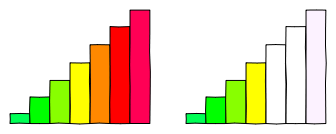
\includegraphics[scale=0.6,keepaspectratio=true]{./activityindicator.png}
\end{figure}
\end{frame}

\begin{frame}
\frametitle{Bausteine}
foo
\end{frame}

\section{Implementierung eines verbesserten Entwicklungsprozesses}

\begin{frame}
\frametitle{Implementierung eines verbesserten Entwicklungsprozesses}
foo
\end{frame}

\begin{frame}
\frametitle{Einf\"uhrungsszenario}
foo
\end{frame}

\begin{frame}
\frametitle{Kommunikation und Kollaboration in einem verteilten Team}
foo
\end{frame}

\begin{frame}
\frametitle{Kollaborativ an einer Vision arbeiten}
foo
\end{frame}

\begin{frame}
\frametitle{Kollaborativ eine Roadmap erstellen}
foo
\end{frame}

\begin{frame}
\frametitle{Qualit\"atssicherung}
foo
\end{frame}

\section{Evaluation}

\begin{frame}
\frametitle{Evaluation}
foo
\end{frame}

\begin{frame}
\frametitle{Umfrage}
foo
\end{frame}

\begin{frame}
\frametitle{Ver\"anderung in der Offenheit des Entwicklungsprozesses}
foo
\end{frame}

\section{Zusammenfassung und Ausblick}

\begin{frame}
\frametitle{Zusammenfassung und Ausblick}
foo
\end{frame}

\end{document}
